\documentclass[12pt,english,british]{article}
\usepackage[affil-it]{authblk}
\usepackage{graphicx}
\usepackage[space]{grffile}
\usepackage{latexsym}
\usepackage{textcomp}
\usepackage{longtable}
\usepackage{multirow,booktabs}
\usepackage{amsfonts,amsmath,amssymb}
\usepackage{url}
%\usepackage[utf8]{inputenc}
\usepackage{hyperref}
\hypersetup{colorlinks=false,pdfborder={0 0 0}}
%\usepackage{latexml}
\newcommand{\truncateit}[1]{\truncate{0.8\textwidth}{#1}}
\newcommand{\scititle}[1]{\title[\truncateit{#1}]{#1}}

\usepackage{lmodern}
\usepackage[T1]{fontenc}
\usepackage[latin9]{inputenc}
\usepackage{geometry}
\geometry{verbose,tmargin=2.5cm,bmargin=2.5cm,lmargin=3cm,rmargin=2.5cm}
\providecommand{\tabularnewline}{\\}
\usepackage[nolist]{acronym}
\newacro{BMI} {body mass index}  
\newacro{LMICs} {low- and middle-income countries}  
\newacro{LMIC} {low- and middle-income country}  
\newacro{MICs} {middle-income countries} 
\newacro{HICs} {high-income countries} 
\newacro{MIC} {middle-income country}  
\newacro{HIC} {high-income country}  
 \newacro{FE} {fixed effects}  
\newacro{HbA1c} {glycated hemoglobin}  
\newacro{IDF} {International Diabetes Federation}  
\newacro{IV} {instrumental variable}  
\newacro{MxFLS} {Mexican Family Life Survey}  
\newacro{OLS} {ordinary least squares}  
\newacro{RE} {random effects}  
\newacro{T2DM} {Type II Diabetes mellitus}  
\newacro{US} {United States}
\newacro{WHO} {World Health Organization} 
\newacro{USA} {United States of America}   
\usepackage{longtable}
\usepackage{booktabs}
%\usepackage{dcolumn}
% Added by lyx2lyx
\usepackage{multirow}
\usepackage{graphicx}
\usepackage[Export]{adjustbox}
%\newcommand{\sym}[1]{\ensuremath{^{#1}}} % for symbols in Table
\usepackage{pdflscape}
\usepackage[authoryear]{natbib}


% paper margins
\usepackage{geometry}
\geometry{
letterpaper,
left=25mm,
right=30mm,
top=20mm,
bottom=30mm,
}   
%limiting tables to only float within section
\usepackage[section]{placeins}
  
%use for commands only working with pdf
  
% formatation

\usepackage{listings}
\lstset{ %
  backgroundcolor=\color{white},   % choose the background color
  basicstyle=\footnotesize,        % size of fonts used for the code
  breaklines=true,                 % automatic line breaking only at whitespace
  captionpos=b,                    % sets the caption-position to bottom
  commentstyle=\color{OliveGreen},    % comment style
  keywordstyle=\color{BlueViolet},       % keyword style
  stringstyle=\color{black},     % string literal style
  language=[AlLaTeX]TeX,             % Set your language (you can change the language for each code-block optionally)
  frame=lrtb, %
  xleftmargin=\fboxsep, %
  xrightmargin=-\fboxsep, %
  moretexcs={lstset,color,colorlet, cellcolor, newcolumntype, columncolor, rowcolor, multirow, xspace, LaTeX, TeX},
}
% *****************************************************************
% Estout related things
% *****************************************************************
\newcommand{\sym}[1]{\rlap{#1}}% Thanks to David Carlisle

\let\estinput=\input% define a new input command so that we can still flatten the document

\newcommand{\estwide}[3]{
		\vspace{.75ex}{
			\begin{tabular*}
			{\textwidth}{@{\hskip\tabcolsep\extracolsep\fill}l*{#2}{#3}}
			\toprule
			\estinput{#1}
			\bottomrule
			\addlinespace[.75ex]
			\end{tabular*}
			}
		}	

\newcommand{\estauto}[3]{
		\vspace{.75ex}{
			\begin{tabular}{l*{#2}{#3}}
			\toprule
			\estinput{#1}
			\bottomrule
			\addlinespace[.75ex]
			\end{tabular}
			}
		}

% Allow line breaks with \\ in specialcells
	\newcommand{\specialcell}[2][c]{%
	\begin{tabular}[#1]{@{}c@{}}#2\end{tabular}}

% *****************************************************************
% Custom subcaptions
% *****************************************************************
% Note/Source/Text after Tables
\newcommand{\figtext}[1]{
	\vspace{-1.9ex}
	\captionsetup{justification=justified,font=footnotesize}
	\caption*{\hspace{6pt}\hangindent=1.5em #1}
	}
\newcommand{\fignote}[1]{\figtext{\emph{Note:~}~#1}}

\newcommand{\figsource}[1]{\figtext{\emph{Source:~}~#1}}

% Add significance note with \starnote
\newcommand{\starnote}{\figtext{* p < 0.1, ** p < 0.05, *** p < 0.01. Robust standard errors in parentheses.}}

% *****************************************************************
% siunitx
% *****************************************************************
\usepackage{siunitx} % centering in tables
	\sisetup{
		detect-mode,
		tight-spacing		= true,
		group-digits		= false ,
		input-signs		= ,
		input-symbols		= ( ) [ ] - + *,
		input-open-uncertainty	= ,
		input-close-uncertainty	= ,
		table-align-text-post	= false
        }


\begin{document}

\title{The impact of diabetes on labor market outcomes in Mexico: a panel and biomarker data analysis}

\author{Till Seuring\footnote{University of East Anglia}, Pieter
Serneels\footnote{University of East Anglia}, Marc Suhrcke\footnote{University
  of York}}
\affil{}

\date{\today}


\maketitle 


\begin{abstract}
Diabetes is increasingly recognized as a major health risk in high income as well as low and middle income countries (LMICs). While adverse economic effects of diabetes are highly plausible, the existing empirical evidence is limited. This paper investigates the effects of diabetes on labor market outcomes focusing on Mexico, a country with high and persistent diabetes rates. Two challenges present themselves when studying this relationship with survey data: (1) causality is hard to identify, and (2) diabetes is typically self-reported, potentially causing biased estimates. This paper makes headway on both fronts using rich panel data. Making use of fixed effects estimation, the analysis accounts for time-invariant omitted variables, providing an improved identification strategy compared to existing work on high income countries. The results indicate a strong negative relationship of self-reported diabetes with probability of employment, which is reduced by 7.5 percentage points. Further, employment probabilities are reduced with each additional year after diagnosis, with the adverse relationship strongest after the first ten years since diagnosis. We find no evidence for an association with wages or working hours. 
Making use of cross-sectional biomarker data from the most recent round to also identify those with undiagnosed diabetes, we find that the adverse relationship remains but is smaller in size, driven by those with self-reported diabetes and finding no associations with undiagnosed diabetes. Together, this indicates that estimates based on self-reported diabetes may overstate the employment effect of diabetes. % Although we cannot rule out that diagnosis itself plays a role, or that people with certain characteristics self-select into diagnosis. 
 


\end{abstract}





\section{\label{sec:Introduction}Introduction }

Diabetes has increased worldwide and is expected to continue to rise over the next decades. It has become a problem for \ac{MICs} and \ac{HICs} alike with over two-thirds of people with diabetes living in the developing world \citep{InternationalDiabetesFederation2013}. Mexicans and Mexican-Americans appear to be particularly affected by diabetes, also in comparison to other Latino populations living in the \ac{US} \citep{Schneiderman2014}. In Mexico itself diabetes prevalence has risen from 6.7 percent in 1994 to 14.4 percent in 2006, including both diagnosed and undiagnosed cases \citep{Barquera2013} and is expected to increase further over the next decades \citep{Meza2015}. Already now, diabetes is the number one cause of death in Mexico. 

This increase in prevalence stems both from a deterioration in diet and a reduction in physical activity \citep{Barquera2008b,Basu2013}, while genetic predisposition among Mexicans with pre-hispanic ancestry also seems to play a role\citep{Williams2013}. Recent evidence indicates that the onset of diabetes increasingly happens at an earlier age in Mexico \citep{Villalpando2010}. With treatment as ineffective as it currently is --- only a minority achieves adequate blood glucose control  \citep{Barquera2013} --- this will increase the likelihood of complications during the productive lifespan. 

Studies for the general \ac{USA} population as well as those focusing on Mexican Americans have found diabetes to be associated with reductions in employment probabilities as well as wages and labor supply \citep{Brown2005,Brown2014,BrownIII2011,Minor2010,Minor2013}.\footnote{ A recent systematic overview also underlines the potential effects on labor market outcomes, as well as individual healthcare expenditures \citep{Seuring2015a}.}
 An earlier cross section analysis for Mexico found a reduction in employment probabilities of 10 percentage points for Mexican men \citep{Seuring2015}. 

However, while these studies have provided good evidence of the potential labor market effects of diabetes, many of the complexities of the relationship have remained unaddressed in this literature. Diabetes is a term used to describe  various diseases characterized by high blood glucose values, with the predominant disease being type II diabetes mellitus, which we will henceforth refer to when using the term diabetes. It is characterized by elevated blood glucose levels due to the body not being able to use insulin properly to maintain blood glucose at normal levels. Elevated blood glucose levels over a prolonged period of time can lead to irreversible health conditions such as heart disease and stroke, blindness, kidney problems, and nerve problems that together with impaired wound healing can lead to the loss of limbs \citep{Reynoso-Noveron2011}. All these conditions can be significantly debilitating and therefore may reduce an individual's economic activity, including his productivity and labor market participation. 

Because diabetes is not a homogeneous disease, it can have distinct effects on people's health, depending on the symptoms and success of disease management. People who are able to "reverse" their diabetes --- meaning they manage to return to healthy blood glucose levels as a result of lifestyle changes and medication that successfully re-establish normal insulin sensitivity --- are unlikely to suffer from any diabetes related health problems \citep{Lim2011, Gregg2012}.
However, if diabetes is either completely untreated or unsuccessfully treated by medical intervention or lifestyle changes, patients are likely to develop the above-mentioned adverse health conditions. The dynamic  aspect of diabetes and the differences in its potential health effects have to be taken into account when investigating its labor market impact. Further, apart from its health effects diabetes might also affect labor market outcomes through other channels. For instance, employers may discriminate against people with diabetes due to their health problems and greater need for medical treatment. Moreover, people aware of their condition may also be less inclined to continue working if this interferes with their disease management; they may also use the diagnosis as a justification for withdrawing from work, i.e. the so called justification bias \citep{Kapteyn2009}. For these reasons the labor market effects may also be distinct for people with diagnosed versus those with undiagnosed diabetes. 

Such sources of unobserved heterogeneity present a challenge to estimate the relationship between diabetes and labor outcomes. Specifically, time-invariant unobserved individual characteristics, like unobserved health endowments --- often related to health during uteru, infant and child years and low household income or adverse health shocks during these early years --- as well as risk preferences have been shown to adversely affect health in general and the propensity to develop type 2 diabetes more specifically \citep{VanEwijk2011,Sotomayor2013,Li2010b}. These and other unobserved personal characteristics (like ability) may also affect employment probabilities, wages or working hours directly through their effects on today's productivity \citep{Currie2013}, as well as indirectly by limiting educational attainment and human capital accumulation \citep{Ayyagari2011a}.

The objective of this study is to provide new evidence on the impact of diabetes on labor outcomes, while improving upon existing estimation by paying close attention to the above challenges. We use three waves  of panel data from Mexico provided by the \ac{MxFLS} covering the years period 2002--2012. The \ac{MxFLS} is particularly useful for the analysis of diabetes and allows us to account for the mentioned complexities in a more refined way than has been the case so far. Using individual level fixed effects analysis for the first time in this literature, we take account of time-invariant heterogeneity when assessing the impact of self-reported diabetes and self-reported diabetes duration on labor market outcomes.\footnote{We are not aware of any other evidence on the effect on wages and working hours in a \ac{MIC}.} Further, we add to the current literature in exploring the role of undiagnosed diabetes, using novel and rich biomarker data - an issue of considerable importance in light of the large prevalence of undiagnosed diabetes (see \citet{Beagley2014}) that remained unaccounted for in all earlier studies relying on self-reported information. Doing so sheds light on the issue of measurement error and the potentially differential effects between diagnosed and undiagnosed diabetes. 

Our  results using self-reported diabetes suggest an economically important decrease in employment probabilities for people aware of their disease. Wages and working hours, however, do not appear to be associated with self-reported diabetes. We further find that employment probabilities are reduced with each additional year since diagnosis, with some evidence for an even larger effect per year after the initial 10 years. 

The biomarker analysis indicates that measurement error of self-reported diabetes leads to an upward biased estimate of the employment penalty, compared to biometrically measured diabetes. Overall, undiagnosed diabetes does not appear to affect any labor market outcome, suggesting that adverse effects mainly occur to those with a diagnosis. 

In general, our results are consistent with the with the dynamic nature of the health effects of diabetes: those with a diagnosis experience an important employment penalty once diagnosed, potentially due to the psychological effects of the diagnosis but presumably also because the condition is typically only diagnosed after several years of asymptomatic but elevated blood glucose levels. In line with this conjecture we find that the adverse effects are stronger several years after diagnosis, likely due to the development of additional and more severe complications.



\section{\label{sec:Labor  outcomes and diabetes literature} Diabetes and labor outcomes -- existing evidence }

Several studies have investigated the effects of diabetes on labor market outcomes. For the US, \citet{Brown2005} estimate  the impact on employment in 1996--1997 in an elderly population of Mexican Americans, living close to the Mexican border, using a bivariate probit model. They find diabetes to be endogenous for women but not for men.  For the latter, the estimates show a significant adverse effect of 7 percentage points. For women, the negative effect becomes insignificant when using IV estimation. 

In another study, again for a Mexican-American sample, \citet{BrownIII2011} look at how diabetes management, inferred from measured \ac{HbA1c} levels, affects employment chances and wages using cross-sectional US data. They find a linear negative association between \ac{HbA1c} levels and both employment chances and wages for men. This particular study does, however, not investigate the effects of undiagnosed diabetes. Two further studies also examine the impact of diabetes on employment and productivity for the US: \citet{Minor2010} focuses on the effect of diabetes on female employment, earnings, working hours and lost work days in the \ac{US} in 2006, finding diabetes to be endogenous and its effect underestimated if exogeneity is assumed. In the \ac{IV} estimates, type 2 diabetes had a significant negative effect on female employment as well as annual earnings but not on working hours. Both studies use a Heckman selection model to adjust for a possible selection bias. However, neither of the studies discusses whether the exclusion restrictions are satisfied. In a later study \citet{Minor2013} investigates the relationship of diabetes duration and labor market outcomes, providing evidence that the relationship is non-linear with employment probabilities declining shortly after diagnosis for men and after about ten years for women; wages are not affected by duration.

For Canada, \citet{Latif2009} estimate the effect of the disease on employment probabilities using an \ac{IV} strategy similar to \citet{Brown2005}. He finds diabetes to be exogenous for females, and both endogenous and overestimated for males in the univariate model, with the estimates of the bivariate model indicate a significant negative impact on the employment probabilities for women, but not for men. 
For Australia, \cite{Zhang2009} analyzes the effects of diabetes on labor force participation using a multivariate endogeneous probit model. They find reduced labor market participation for males and females. They also find that if the endogeneity of diabetes is unaccounted for, effects are overstated. 

Only two studies exist for \ac{MICs} by our knowledge. \citet{Liu2014} investigate the effect of diabetes diagnosis on labor income in China, exploiting a natural experiment to identify causality and find a significant reduction in income for those with a recent diagnosis. An earlier study for Mexico, investigated the effect of self-reported diabetes on the probability of employment using cross-sectional data from the 2005 wave of the \ac{MxFLS}, and found a significant (p<0.01) reduction in employment chances for males by about 10 percentage points and for females by about 4.5 (p<0.1) percentage points, using parental diabetes as an \ac{IV} \citep{Seuring2015}. The scarcity of evidence for \ac{LMICs} is also underlined in a recent systematic review of the economic cost of diabetes \citep{Seuring2015a}. 


Overall, the majority of existing studies, including those on high income countries, seem to suffer from at least three key limitations: 
\begin{enumerate}
\item  They rely exclusively on cross-sectional data, unable to account for unobserved characteristics.
\item The use of the family history of diabetes, which has been the sole instrumental variable employed so far, relies on the finding that type 2 diabetes has a genetic and heritable component that could theoretically provide valid identification of the true effect of diabetes. However, it remains unclear whether the variable fully satisfies the exclusion restriction, as it may also proxy for other genetically transferred traits, including those that impact labor outcomes directly, as for instance unobserved abilities. This traditional identification strategy also abstracts from intrahousehold or intergenerational labor supply effects \citep{Seuring2015}.\footnote{It is conceivable that diabetes might deteriorate parental health in such a way that the offspring either has to give
up their employment to provide care, or has to increase labor supply to compensate for lost income.}
\item The use of self-reported diabetes can introduce non-classical measurement error due to systematic misreporting which has been shown to cause estimates of economic impacts to be potentially biased and overstated  \citep{Cawley2015,ONeill2013,Perks2015}.
\end{enumerate}


As mentioned before, to overcome some of these these limitations, this paper applies a individual level \ac{FE} panel estimation strategy and biomarker data. It also goes into more detail by estimating models according to the type of employment, i.e. non-agricultural employment, agricultural employment and self-employment, as ill health may have distinct effects across these activities.




\section{\label{sec:Data}Data}

We use the \acf{MxFLS}, a nationally representative, longitudinal household survey, which has three
waves, conducted in 2002, 2005--2006 and 2009--2012. All household members aged 15 and above were interviewed, covering information on a wide range of social, demographic, economic characteristics and
health behaviours of the individuals and their families
\citep{Rubalcava2013}. Apart from self-reported diabetes information that is available in all rounds, we also use information
on the self-reported year of diagnosis as well as biomarker data including \ac{HbA1c} levels for a subsample of respondents.  Our main analysis uses all three waves 
taking advantage of the large amount of observations (N=49,323) and the panel structure
of the data. Our variable of interest is self-reported
diabetes, which is based on the survey question: "Have you
ever been diagnosed with diabetes?". 


However, the response to this question may well suffer from measurement error, possibly depending on how long ago the diagnosis took place (if it did) and, perhaps more importantly, on whether the respondent was communicated the result and is aware that he or she has the disease. The possible challenges for self-reported data are reflected in the observed inconsistencies in the self-reports for the same individuals across rounds. 
We investigate and try to correct the self-reported diabetes variable for these inconsistencies, using disease information from previous and future waves to infer on the missing diabetes status (See Appendix \ref{sec:Appendix} for further details on our correction procedures.)  This approach is, however, unable to address the no less important problem of undiagnosed diabetes. In order to investigate how such measurement error may affect estimates of the labor market impact of diabetes
we use the information from a subsample containing over 6000 respondents (everybody aged 45+  and a random subsample of those aged 15--44 \citep{Crimmins2015}) of the 2009-2012 wave, allowing us to use biometrically measured diabetes to identify those with undiagnosed diabetes. For the entire paper the samples we use are restricted to the working age population (15--64). To prevent pregnant women from biasing our results due to the increased diabetes risk during pregnancy and its effects on female employment status, we have dropped all observations of women reporting to be pregnant at the time of the survey (N=764).


The detailed information in the \ac{MxFLS} allows us to construct the following outcome variables of interest: employment, hourly wage and weekly working hours \footnote{Hourly wage was calculated by adding up the reported monthly income from the first and potential second job and dividing it by the average number of weeks per month. This gave us the average earnings per week which was then divided by the weekly working hours to arrive at an hourly wage estimate. Labor income was either reported as the total amount for the whole month or if possible more detailed containing information on the monthly wage, income from piecework, tips, extra hours, meals, housing, transport, medical benefits and other earnings. Over 80 percent of respondents reported the total amount instead of a detailed amount. Respondents were also asked for their yearly income and we used that information to arrive at an hourly wage if information for monthly labor income was missing. Finally, we adjusted the calculated wage for inflation from the year of the interview up to 2013 and logarithmized the  values. Due to a considerable number of missing or zero income reports the sample used for the wage estimation is smaller than the sample for working hours. Working hours were calculated summing up the self-reported usual working hours of the first and potential second job. We dropped 39 observations where the sum of working hours exceeded 112 hours per week, i.e. more than 16 hours of work per day on each day of the week as we deemed these reports to be unrealistic.}. Regarding diabetes, unweighted self-reported diabetes prevalence in the \ac{MxFLS} increased from about 6 percent in 2002 to 7.1 percent in 2009 for females and from about 4.3 to 5.7 percent for males. This is below estimates for Mexico from other institutions, who, however, include undiagnosed diabetes in their estimates. \citet{Barquera2013} show that the prevalence of diagnosed diabetes in Mexico was 7.5 percent in 2006, only somewhat above our results, which may be the result of the slightly different age groups analyzed.\footnote{Including undiagnosed diabetes, the overall prevalence was 14.4 percent in 2006.}  For the pooled data of all three waves (Table  \ref{tab:Pooled-sample-characteristics}),
diabetes was self-reported by 5 percent of men and 6.2 percent of
women. Most of the respondents in the sample either live in rural
or in large urbanized areas. Looking at our outcome variables, 86
percent of men report some form of employment compared to 36 percent
of women. Interestingly, men do not report higher hourly wages compared
to women but work more hours per week. Also, men are working more
often in agricultural jobs while women are more likely to be self-employed
or in non-agricultural employment. Women also have lower educational
attainment on average. 



\begin{table}[!ht]
\caption{\label{tab:Pooled-sample-characteristics}Means  for pooled sample (2002, 2005-2006, 2009--2012) and biomarker sample (2009--2012) with standard deviations in parenthesis}
\begin{center}

\begin{adjustbox}{max width=\textwidth}
{
\def\sym#1{\ifmmode^{#1}\else\(^{#1}\)\fi}
\begin{tabular}{l*{4}{cc}}
\toprule
                    &\multicolumn{4}{c}{Panel}                          &\multicolumn{4}{c}{Biomarker}                      \\\cmidrule(lr){2-5}\cmidrule(lr){6-9}
                    &\multicolumn{2}{c}{Males}&\multicolumn{2}{c}{Females}&\multicolumn{2}{c}{Males}&\multicolumn{2}{c}{Females}\\
\midrule
\hspace*{10mm}\emph{Dependent variables}&& \\
Employed            &        0.87&      (0.34)&        0.37&      (0.48)&        0.86&      (0.35)&        0.34&      (0.47)\\
Hourly wage             &       42.20&    (485.24)&       41.28&    (169.35)&       36.27&     (53.63)&       35.29&     (43.66)\\
Usual weekly working hours &       46.81&     (16.79)&       39.00&     (18.91)&       45.98&     (16.89)&       38.18&     (19.66)\\
Agricultural worker &        0.22&      (0.41)&        0.04&      (0.20)&        0.25&      (0.43)&        0.03&      (0.18)\\
Self-employed       &        0.19&      (0.39)&        0.28&      (0.45)&        0.21&      (0.41)&        0.32&      (0.47)\\
Non-agricultural worker or employee&        0.59&      (0.49)&        0.68&      (0.47)&        0.53&      (0.50)&        0.64&      (0.48)\\
\hspace*{10mm}\emph{Diabetes variables}&&&& \\
Diagnosed diabetes  &        0.05&      (0.22)&        0.06&      (0.24)&        0.09&      (0.29)&        0.12&      (0.32)\\
Diabetes duration   &        0.34&      (2.00)&        0.42&      (2.38)&        0.67&      (2.81)&        0.88&      (3.41)\\
Glycated hemoglobin (HbA1c)&            &            &            &            &        6.46&      (1.88)&        6.58&      (2.02)\\
HbA1c $\geq 6.5\%$  &            &            &            &            &        0.26&      (0.44)&        0.28&      (0.45)\\
Undiagnosed diabetes&            &            &            &            &        0.18&      (0.39)&        0.18&      (0.39)\\
\hspace*{10mm}\emph{Education and demographic variables}&&&& \\
Age                 &       36.03&     (13.62)&       36.28&     (13.17)&       42.78&     (14.28)&       42.78&     (13.95)\\
Rural&        0.44&      (0.50)&        0.43&      (0.50)&        0.51&      (0.50)&        0.46&      (0.50)\\
Married             &        0.54&      (0.50)&        0.54&      (0.50)&        0.60&      (0.49)&        0.56&      (0.50)\\
Number of children (age<6)&        0.56&      (0.82)&        0.61&      (0.85)&        0.49&      (0.79)&        0.53&      (0.82)\\
Indigenous group    &        0.19&      (0.39)&        0.19&      (0.39)&        0.19&      (0.39)&        0.18&      (0.39)\\
Secondary           &        0.30&      (0.46)&        0.30&      (0.46)&        0.26&      (0.44)&        0.26&      (0.44)\\
High school         &        0.16&      (0.36)&        0.13&      (0.34)&        0.14&      (0.34)&        0.12&      (0.33)\\
Higher education    &        0.11&      (0.32)&        0.09&      (0.29)&        0.12&      (0.32)&        0.09&      (0.28)\\
\midrule
Observations        &       21438&            &       27412&            &        2795&            &        3632&            \\
\bottomrule
\multicolumn{9}{l}{\footnotesize Results for the other control variables, i.e. the Mexican states, log hourly wage and wealth, are omitted to save space.}\\
\end{tabular}
}
\end{adjustbox}
\end{center}
\end{table}

Turning to the biomarker subsample of the third wave (2009-2012), it is important to note that in this subsample respondents are somewhat older on average than in the pooled sample, as it includes everybody above the age of 44 but only a random subsample of those aged 44 or below (\cite{Crimmins2015}). Also, self-reported diabetes is considerably higher than in the pooled sample as well as in the full sample of wave 3. Regarding the other control and outcome variables, the sample is fairly similar to the pooled sample. The added value of this subsample is in the biomarker information regarding diabetes. A large share of the subsample has an \ac{HbA1c} indicative of diabetes.\footnote{In one of the first analyzes of these new biomarker data \citet{Frankenberg2015} show that the rates in Mexico of elevated \ac{HbA1c} levels are very high when compared to \ac{HbA1c} data from similar surveys in the \ac{USA} and China. This study also notes that "The extremely high levels of elevated \ac{HbA1c} among Mexicans adults (...) is profoundly troubling." \citep[p.18]{Frankenberg2015}.} In our Mexican sample, over 18 percent of males and females result as having undiagnosed diabetes. These first descriptive results suggest that using self-reported diabetes as a measure for diabetes in Mexico can lead to a strong underestimate of the true diabetes population. In the following sections we will therefore shed some light on how taking the large undiagnosed population into account could affect the impact estimates of diabetes on labor outcomes. 

\section{\label{sec:Estimation Strategy}Estimation strategy}

  
The conceptual framework of our study is based on the work of \citet{Strauss1998}, who specify the following model of the relationship between health and labor market outcomes, i.e. labor force participation and labor supply conditional on health and wages.
\begin{equation}
L=L(H, pc, w(H;S,A,B,I,\alpha,e_{w}), S, A, B, V, \xi) \label{eq:wage}
\end{equation}
where $L$ is labor supply or labor market participation, $pc $ is a vector of prices for consumer goods, $w$ is the real wage; $H$ is an array of measured health human capital ; $S$ is education; $A$ is a vector of demographic characteristics; $B$ is the family background of the individual; $I$captures the local community infrastructure; $\alpha$ is an array of unobservables (e.g. ability), $e_w$ represents the measurement error, $V$ is non-labor income and $\xi$ is the taste parameter. 

The equation showcases the joint effect of health on both wages and labor supply or labor market participation. Health affects labor supply and participation indirectly by changing wages and directly by impacting the ability to work.

There are several ways diabetes may affect $H$. First of all, diabetes can deteriorate health if it remains untreated with the adverse effects potentially increasing over time. Second, a diagnosis of diabetes and ensuing treatment may lead to better health compared to the undiagnosed state. However, compared to healthy people even those with diabetes receiving treatment may still have worse health outcomes. Third, there is also evidence that the diagnosis itself may affect one's own health perception and can lead to worse self-perceived health \citep{Thoolen2006a}. We therefore expect diabetes to adversely affect health and consequently labor market outcomes.

When estimating equation  \ref{eq:wage} empirically with observational data, unobserved heterogeneity may bias the results. As mentioned in section  \ref{sec:Introduction} unobserved factors captured in $\alpha$ such as early childhood investments, innate ability and time preference could affect wages as well as the probability to develop diabetes. Further, changes in lifestyle due to changes in wages or employment status may also affect the probability to develop diabetes through changes in diet and physical activity. Finally, measurement error $e_w$ may be an important issue due to the large undiagnosed population with diabetes, particularly if being diagnosed is related to employment or wages via better access to healthcare through employment benefits and higher income.

The following section describes our estimation strategy.


\subsection{Panel data estimation strategy: Self-reported Diabetes}

We investigate the relationship of self-reported diabetes and three
labor market outcomes: employment, wages and labour supply , respectively, using a fixed effects model. While using individual level \ac{FE} does not allow to fully
identify a causal relationship, this strategy does improve on the degree of causal inference,
compared to a simple cross-sectional analysis.\footnote{Other forms of unobserved heterogeneity could also
affect our estimates - for instance time-variant unobserved heterogeneity
or omitted variables simultaneously driving labor outcomes and health} In particular it
does allow controlling for unobserved personal characteristics that
could bias the estimates, without the drawbacks of a less than convincing
\ac{IV} strategy that has been widely applied in this literature. We have also estimated \ac{RE} models but do not present them here as the Hausman test suggested the use of the \ac{FE} model throughout.\footnote{Results are available on request.}


We estimate the following model:

\noindent 
\begin{equation}
Y_{it}=\beta_{0}+\beta_{1}Diabetes_{it}+\beta_{2}X_{it}+c_{i}+\gamma_{t}+u_{it}.\label{eq:employed}
\end{equation}


where $Y_{it}$ is a binary variable taking a value of $1$ if respondent
$i$ reports being employed at time $t$ and $0$ otherwise, $Diabetes_{it}$
is a binary variable taking a value of $1$ at time $t$ if the respondent
reports having ever received a diagnosis of diabetes, $X_{it}$ is
a vector of control variables, $c_{i}$ represents an individual fixed
effect, $\gamma_{t}$ represents a year fixed effect, and $u_{it}$
is the error term.

For the relationship of self-reported diabetes with log hourly wages
and weekly working hours our empirical models are estimated conditional on having positive wages and being
employed, respectively. In these models $Y_{it}$ represents the log hourly wage
of respondent $i$ at time $t$ or the usual weekly working hours
over the last year.

The control variables in both \ac{FE} specifications include dummy variables for the effects of any changes in the living environment,
of living in a small, medium or large city with rural as the reference category, and state
dummies capturing the effects of moving to a different state. We also include a marital
status dummy to control for the impact of marriage on the probability of being employed.
A variable capturing the number of children residing in the household
below the age of 18 is used to control for the impact of children
on labor market outcomes and the effect of childbearing and related
gestational diabetes on the probability of developing type 2 diabetes
\citep{Bellamy2009}. To account for the effect that changes in household
wealth might have on diabetes and employment probabilities, we use standard
principal component analysis of multiple indicators of household assets
and housing conditions to create an indicator for household wealth
\citep{Filmer2001}.\footnote{The components used for the construction of the
wealth index are detailed in \citet{Seuring2015}}. Finally, calender year fixed effects are included to capture the effects of increasing age and of any macroeconomic shocks over time.

To explore the role of the duration of diabetes for labor outcomes, we estimate the following model using a self-reported
measure of the years since diagnosis:


\begin{equation}
Y_{it}=\beta_{0}+\beta_{1}Dyears_{it}+\beta_{2}X_{it}+c_{i}+\gamma_{t}+u_{it},\label{eq:duration_linear}
\end{equation}


\noindent where $\beta_{1}Dyears_{it}$ is a continuous variable indicating
years since first diabetes diagnosis.

In an effort to capture possible non-linearities in the relationship of interest we then use a spline function that allows the effect
of an additional year with diabetes to vary over time.
\begin{equation}
Y_{it}=\delta_{0}+g(Dyears_{it})+\delta_{2}X_{it}+c_{i}+\gamma_{t}+u_{it}.\label{eq:splines}
\end{equation}


\noindent with $g(Dyears_{it})=\sum_{n=1}^{N}\delta_{n}\cdot max\{Dyears_{it}-\eta_{n-1}\}I_{in}$
and $I_{in}=1[\eta_{n-1}\leq Dyears_{it}<\eta_{n}]$, with $\eta_{n}$
being the place of the $n$-th node for $n=1,2,\ldots,N$. We choose
three nodes that - based on visual inspection (see Figures \ref{fig:Kernel-weighted-local-polynomial_empl}, \ref{fig:Kernel-weighted-local-polynomial_wage} and \ref{fig:Kernel-weighted-local-polynomial_workhrs} in the
result section) - best captured any possible non-linearity in the
relationship between diabetes duration and labor outcomes. These
are located at four, eleven and twenty years after diagnosis. The
first four years should capture any immediate effects of the diagnosis,
the years five to eleven should capture any effects of adaptation to
the disease. After eleven years it is conceivable that many of the
debilitating complications of diabetes would appear that could deteriorate
health and lead to adverse effects on labor market outcomes.
The coefficient $\delta_{n}$ captures the effect of diabetes for the
$n$-th interval. The effects are linear if $\delta_{1}=\delta_{2}=,\ldots,=\delta_{n}$.

Because the year of diagnosis was only reported in the third wave,
duration of diabetes (or time since diagnosis)
for the earlier waves was only calculated for those that had also responded to the third
wave. To arrive at the time passed since diagnosis, the year of diagnosis
was subtracted from the year of the interview. %In order to have zero years representing people without a self-reported diagnosis, those that reported a diagnosis in the year of the interview were counted as 'one year since diagnosis'. Accordingly, if the respondent reported to having been diagnosed in the year before the interview he or she was counted as 'two years since diagnosis' and so on.

In a fixed effects estimation, when year dummies are included, any variable that varies by one
unit in each time period, such as age, is not separately identified, while any non-linear term is obviously identified. Diabetes duration, in equations (\ref{eq:duration_linear}) and (\ref{eq:splines}), also increases by one unit each
year, like age, but it is interacted with the diabetes dummy, which takes value zero for individuals
who are not retired. Hence identification of this variable relies on the presence in the sample of people without diabetes. Consequently, those that reported a diagnosis in the year of the interview were counted as 'one year since diagnosis'. From this follows that if the respondent reported to having been diagnosed in the year before the interview he or she was counted as 'two years since diagnosis' and so on. (need to rewrite this a bit as it is taken more or less from http://www.netspar.nl/files/Evenementen/2015-01-28-30/086%20Borella.pdf). There might be some further studies in the retirement literature that could be used as reference for this approach.



\subsection{Cross-section data estimation strategy: biomarker and self-reported data}

Self-reported diabetes only captures part of the diabetes population as many individuals remain undiagnosed.  Estimations based on self-reports may therefore suffer from a selection bias.

Self-reports of diabetes can lead to errors due to two main factors: 
\begin{enumerate}
\item Systematic overreporting of diabetes: people without diabetes
could intentionally report a diabetes diagnosis with a view to justifying
some other adverse event or status in their life (e.g. being unemployed). 
\item Systematic underreporting of diabetes: it is also conceivable
that people with diabetes are concerned about negative stigma associated with the condition, resulting in underreporting. Further, diabetes often remains
undiagnosed for long periods of time or may remain undiagnosed altogether, potentially
leaving many people unaware of the disease, hence resulting in
underreporting.\footnote{The issue of measurement error can be depicted transparently in a stylized way. Assume that the true model of the effect of diabetes on labor market outcomes is $y^{*}=X^{*}\beta+\epsilon$. Because we do not observe the true values of $y^{*}$ and $X^{*}$  we have to use reported measures that contain errors: $X=X^{*} + u$ and $y=y^{*} + v$. In the case of diabetes as a right-hand side variable, this measurement error is negatively correlated with the true diabetes status, in contrast to classic measurement error which is randomly distributed. Hence, the direction of the bias is unknown and cannot be assumed to be attenuating.}

\end{enumerate} 

Overreporting may attenuate the coefficient of diabetes as those falsely reporting a diabetes diagnosis experience no adverse health
effects of diabetes that could affect labor outcomes. However, if some of those misreports are
made in order to justify some other adverse event, e.g. current unemployment
or other health problems, then this could lead to an upward bias
of the estimated effect of diabetes on employment. Underreporing due to
a non-diagnosis may cause either an overestimation or attenuation
bias: it leads to an overestimation if those with undiagnosed
diabetes are generally healthier, hence more likely to have
positive labor market outcomes than those with diagnosed diabetes. However, if the undiagnosed and the diagnosed groups are similar in terms of health, then this leads to an attenuation of the diabetes coefficient. This is because the control group is less healthy, because it includes the undiagnosed, and consequently has worse labor outcomes then it would have if all diabetes cases were diagnosed.

An important additional issue may arise due to the health information received at a diabetes diagnosis. More specifically, a diabetes diagnosis likely also affects an individual's psychology and
behavior which in turn may have its own effects on economic
outcomes. So did studies find a diabetes diagnosis and subsequent treatment
to increase the odds of psychological problems, including depression
and anxiety \citep{Thoolen2006a,Paddison_2011}.
Interestingly, similar results have not been found for people with
undiagnosed diabetes \citep{Nouwen2011}. Looking at behavioral change, health information  has been shown to affect behavior after the diagnosis of diabetes \citep{Slade2012} and of other chronic diseases as well (see \citep{Baird2014,Gong2015,Thornton2008,Zhao2013a}).There is, however, little research on the effects of health information on labor market outcomes. For diabetes, only \citet{Liu2014} investigate the effect of receiving a diabetes diagnosis on labor income in Chinese employees and found that a recent diagnosis reduced labor income potentially due to it psychological effects. 
Finally, if the decision to supply work is also affected by the own health perception, information on a person's diabetes status can affect labor choices. If a person had previously experienced symptoms, he or she may now find relief in the ability to treat the disease and may increase labor supply if the symptoms disappear. Or, if diabetes had been asymptomatic before diagnosis, then he or she may reduce labor supply as a reaction to the worse than expected health status.  

We use the biomarker data in wave three to explore the relationship of measured diabetes, including undiagnosed diabetes with labor outcomes and compare it to estimates using self-reported diabetes. The biomarker data also allows us to look at diabetes severity, as measured
by \ac{HbA1c} values. Since this data is only available for one wave -- the
last wave -- our analysis here is limited to cross-section data. Moreover,
as mentioned above, biomarkers were only taken from about one-third  of the initial representative sample, which leaves
us with information on 6427 survey participants -- still a sizable number but no longer directly comparable to the panel-based results in this paper.
Nonetheless, it allows for a first exploration of the relationships
of undiagnosed diabetes and disease severity with labor market
outcomes. We first estimate a model to investigate the association of biometrically  
measured diabetes (HbA1c $\geq6.5\%$) with labor market outcomes: 
\begin{equation}
Y_{i}=\beta_{0}+\beta_{1}Dbiom_{i}+\beta_{2}X_{i}+c_{i}+u_{i}\label{eq:diab_objective}
\end{equation}
where $\beta_{1}Dbiom_{i}$ is equal to $1$ if HbA1c $\geq6.5\%$.
In a further step we estimate the following equation 
\begin{equation}
Y_{i}=\beta_{0}+\beta_{1}Dsr_{i}+\beta_{1}Dud_{i}+\beta_{2}X_{i}+u_{i}.\label{eq:diab_sr_ud}
\end{equation}
to investigate how the associations differ between people with diagnosed
and undiagnosed diabetes. $\beta_{1}Dsr_{i}$ identifies the effect of those diagnosed
and is equal to $1$ if the person self-reported a diabetes diagnosis.
$\beta_{1}Dud_{i}$ identifies the effect of those undiagnosed and is equal to $1$
if the person did not self-report a diabetes diagnosis but has an
HbA1c $\geq6.5\%$. Importantly, we include in all models using the biomarker data community fixed effects $c_{i}$ to account for unobserved community characteristics, such as the access to healthcare and the quality of healthcare in the community, poverty and unemployment levels in the community or the amount of public green space and recreational possibilities available. These factors could potentially affect the propensity to (1) develop diabetes and (2) to receive a diagnosis of diabetes, plus they may affect labor market outcomes.\footnote{We did not use household fixed effects as the average number of observations per household was close to one, i.e. for most households only one member provided biomarker information in our subsample, significantly limiting the variation within households that would be needed for identification.}

Before moving on to the results it bears emphasizing that despite our efforts to reduce any bias in our estimates, the degree of causal inference we can make remains limited. While the fixed effects model accounts for time invariant
unobserved confounders, it is still possible that the estimates are biased
due to time variant heterogeneity which the estimated models do not account for. For instance, job loss may affect lifestyle choices that increase the probability to develop
diabetes which could then in turn negatively affect labor market outcomes. So far, no strong adverse effects of being laid
off on diabetes self-reports have been found in the literature \citep{Bergemann2011,Schaller2015},
although this has only been researched in a high-income country context.  Further, stress at work has been linked to the development of type 2 diabetes \citep{Heraclides2012,Eriksson2013}, presenting another potential confounder. However, we argue that the fixed effects approach should limit the potential confounding as the main characteristics that could affect a person's diabetes probabilities as well as stress levels, genetic predisposition to diabetes and stress coping mechanisms (see \citet{Schneiderman2005}), are likely time-invariant. Nonetheless, it may still be the case that other forms of unobserved heterogeneity bias the estimates.


\section{\label{sec:RESULTS} Results}


\subsection{Panel data analysis}

\subsubsection{Incidence of self-reported diabetes}

Table \ref{tab:Self-reported-diabetes-and} presents the estimation
results of the \ac{FE} model using equation \ref{eq:employed} .
The results indicate significant and substantial reductions in the probability of employment
for men and women with self-reported diabetes. The effects are surprisingly similar across both sexes showing a reduction in
employment probabilities of around 7 percentage points. 
\begin{table}[h]
\caption{\label{tab:Self-reported-diabetes-and}Self-reported diabetes and labor market outcomes}
\begin{center}
%\resizebox{\textwidth}{!}{%
\begin{adjustbox}{max width=\textwidth}
{
\def\sym#1{\ifmmode^{#1}\else\(^{#1}\)\fi} \begin{tabular}{l*{6}{SS}}
\toprule
                &\multicolumn{2}{c}{Employment}       &\multicolumn{2}{c}{Log hourly wages} &\multicolumn{2}{c}{Monthly work hours}\\\cmidrule(lr){2-3}\cmidrule(lr){4-5}\cmidrule(lr){6-7}
                &\multicolumn{1}{c}{(1)}&\multicolumn{1}{c}{(2)}&\multicolumn{1}{c}{(3)}&\multicolumn{1}{c}{(4)}&\multicolumn{1}{c}{(5)}&\multicolumn{1}{c}{(6)}\\
                &\multicolumn{1}{c}{Males}&\multicolumn{1}{c}{Females}&\multicolumn{1}{c}{Males}&\multicolumn{1}{c}{Females}&\multicolumn{1}{c}{Males}&\multicolumn{1}{c}{Females}\\
\midrule
Diagnosed diabetes&    -.075\sym{***}&    -.071\sym{***}&     .010         &     .074         &    -.945         &   -2.158         \\
                &   (.025)         &   (.024)         &   (.067)         &   (.157)         &  (1.505)         &  (2.516)         \\
\midrule
R2 within             &     .011         &     .017         &     .016         &     .032         &     .010         &     .019         \\
N               &    21400         &    27365         &    13833         &     7076         &    17625         &     9123         \\
\bottomrule
\multicolumn{7}{l}{\footnotesize Fixed effects estimation; robust standard errors in parentheses.}\\
\multicolumn{7}{l}{\footnotesize Other control variables: state dummies, urbanization dummies, education dummies, married dummy, number children < 6}\\
\multicolumn{7}{l}{\footnotesize wealth, age and calender year fixed effects.}\\
\multicolumn{7}{l}{\footnotesize The wage and working hour models additionally control for type of work (agricultural and self employed with}\\
\multicolumn{7}{l}{\footnotesize non-agricultural employment as the base) and for health insurance status.}\\
\multicolumn{7}{l}{\footnotesize \sym{*} \(p<0.10\), \sym{**} \(p<0.05\), \sym{***} \(p<0.01\).}\\
\end{tabular}%
}
%}
\end{adjustbox}
\end{center}
\end{table}

The results in Column 3 indicate no significant relationship between self-reported diabetes and
wages or working hours.

To investigate this same relationship across different types of work, we estimate
a model including interaction terms between self-reported diabetes
and agricultural employment and between self-reported diabetes and
self-employment, respectively, using non-agricultural employment as
the comparison group. One may expect this relationship to differ by the type of work, as
those  with diabetes working in an agricultural job that requires strenuous,
physical efforts may see their productivity more adversely affected than those engaged in more sedentary work. 


\begin{table}[!ht]
\caption{\label{tab:Self-reported-diabetes-interaction}Relationship between self-reported diabetes by type of work and wages and working hours}
\begin{center}
%\resizebox{\textwidth}{!}{%
\begin{adjustbox}{max width=\textwidth}
{
\def\sym#1{\ifmmode^{#1}\else\(^{#1}\)\fi}
\begin{tabular}{l*{4}{SS}}
\toprule
                &\multicolumn{2}{c}{Log hourly wage}&\multicolumn{2}{c}{Monthly work hours}\\\cmidrule(lr){2-3}\cmidrule(lr){4-5}
                &\multicolumn{1}{c}{(1)}&\multicolumn{1}{c}{(2)}&\multicolumn{1}{c}{(3)}&\multicolumn{1}{c}{(4)}\\
                &\multicolumn{1}{c}{Males}&\multicolumn{1}{c}{Females}&\multicolumn{1}{c}{Males}&\multicolumn{1}{c}{Females}\\
Reference category: Non-agricultural employee&&&& \\ \\
Agricultural worker&    -.079\sym{*}  &    -.283         &   -3.534\sym{***}&   -4.658\sym{*}  \\
                &   (.044)         &   (.186)         &   (.799)         &  (2.708)         \\
Self-employed   &     .038         &    -.139         &   -1.438\sym{**} &   -4.696\sym{***}\\
                &   (.043)         &   (.087)         &   (.705)         &  (1.383)         \\
Diagnosed diabetes&     .071         &     .058         &     .294         &    -.765         \\
                &   (.075)         &   (.168)         &  (1.605)         &  (2.250)         \\
Diagnosed diabetes x agricultural worker&    -.282         &    -.397         &   -5.772\sym{**} &   -2.795         \\
                &   (.188)         &   (.371)         &  (2.848)         & (22.248)         \\
Diagnosed diabetes x self-employed&    -.129         &     .120         &     .186         &   -4.054         \\
                &   (.204)         &   (.323)         &  (2.513)         &  (4.744)         \\
\midrule
R2 within           &     .016         &     .032         &     .011         &     .019         \\
N               &    13833         &     7076         &    17625         &     9123         \\
\bottomrule
\multicolumn{5}{l}{\footnotesize Fixed effects estimation; robust standard errors in parentheses.}\\
\multicolumn{5}{l}{\footnotesize Other control variables: state dummies, urbanization dummies, education dummies, married dummy, number children < 6,}\\
\multicolumn{5}{l}{\footnotesize  wealth, health insurance status, age and calender year fixed effects.}\\
\multicolumn{5}{l}{\footnotesize \sym{*} \(p<0.10\), \sym{**} \(p<0.05\), \sym{***} \(p<0.01\).}\\
\end{tabular}
}
%}
\end{adjustbox}
\end{center}
\end{table}  

\FloatBarrier
  
The results in Table \ref{tab:Self-reported-diabetes-interaction} shows that while male
agricultural workers have lower wages in general, the relationship
with diabetes does not depend on the type of work, as none of the interaction terms shows up significant. In the working hours regression one interaction term is significant, suggesting that those with self reported diabetes working in agriculture supply x less hours relative to non-agricultural workers and employees. The only
statistically more relevant relationship that we find relates to working
hours of agricultural workers with diabetes, who appear to work about
five hours less than non-agricultural workers without self-reported diabetes.
However, because we have more than two work types we cannot draw conclusions
solely on the basis of the t-statistic. We therefore perform a Wald
test for the overall significance of the interaction term which does
not reject the null of no interaction effects, suggesting that the
effect of diabetes on working hours does not vary significantly by type of work.  Overall, we find no evidence for an association between self-reported diabetes and wages or working hours, in line with \citet{Minor2013}, who does not find strong evidence for any effects beyond those on employment (though he does not look at working hours). The lack of effects at the intensive margin may be explained by selection. Potentially, only those with "mild" or asymptomatic diabetes are still in employment continuing to earn similar wages. Additionally, some of them may also resort to different, less physically demanding, activities within the workplace allowing them to maintain employed. Only once complications become increasingly severe would they drop out of the labor market, without going through a notable phase of reduced productivity and labor supply. 

Finally, we explore whether diabetes affects the selection into type of work. One approach to test this would be to use a \ac{FE} multinomial logit model. Because of ambiguity surrounding the calculation of interpretable marginal effects in this model \citep{Pforr2014}, we instead estimate \ac{FE} models of the probability of being in non-agricultural employment, agricultural employment or self-employment using three dummy variables indicating the respective type of work as the dependent variable.\footnote{For example, "non-agricultural employment" is coded as $1$ if the respondent is engaged in agricultural work and is coded as $0$ for those unemployed, in non-agricultural employment or self-employed. This is repeated for the dummy variables "agricultural employment" and "self-employed".} The results in Table \ref{tab:Self-reported-diabetes-selection_LPM} show that for men diabetes mainly appears to be associated with a reduced probability to be self-employed, while for women, those who self report diabetes are less likely to work in either agriculture and self-employment. This may suggest that having diabetes drives people out of self-employment and agricultural jobs, for instance because these jobs are physically more demanding and possibly also because they provide less protection in terms of insurance and employment duration. We interpret the fact that the coefficient signs are negative for all types of work as a confirmation of the earlier result that people with diabetes have predominantly lower employment probabilities.

Finally, before proceeding to further analysis, we need to emphasize that our fixed effects strategy used to identify the effect of self-reported diabetes relies on those reporting a new diabetes diagnosis between any of the waves, which disregards people that have had diabetes before the start of the survey and so limits the estimation of effects to those more or less recently diagnosed. Accordingly, the obtained results may be different from those with a longer disease history. \footnote{However, at least the results of the \ac{RE} analysis (available on request), which also includes between-person variation, do not indicate that the effects are substantially different even when people with a longer disease history are taken into account.}. 


\begin{table}[h]
\caption{\label{tab:Self-reported-diabetes-selection_LPM}Relationship between self-reported diabetes with selection into types of work}
\begin{center}
%\resizebox{\textwidth}{!}{%
\begin{adjustbox}{max width=\textwidth}
{
\def\sym#1{\ifmmode^{#1}\else\(^{#1}\)\fi}
\begin{tabular}{l*{6}{S
S}}
\toprule
                &\multicolumn{3}{c}{Males}                               &\multicolumn{3}{c}{Females}                             \\\cmidrule(lr){2-4}\cmidrule(lr){5-7}
                &\multicolumn{1}{c}{(1)}&\multicolumn{1}{c}{(2)}&\multicolumn{1}{c}{(3)}&\multicolumn{1}{c}{(4)}&\multicolumn{1}{c}{(5)}&\multicolumn{1}{c}{(6)}\\
                &\multicolumn{1}{c}{Non-agric.}&\multicolumn{1}{c}{Agric.}&\multicolumn{1}{c}{Self-employed}&\multicolumn{1}{c}{Non-agric.}&\multicolumn{1}{c}{Agric.}&\multicolumn{1}{c}{Self-employed}\\
\midrule
Diagnosed diabetes&    -.021         &    -.009         &    -.050\sym{*}  &    -.009         &    -.022\sym{***}&    -.033\sym{*}  \\
                &   (.029)         &   (.021)         &   (.026)         &   (.018)         &   (.009)         &   (.018)         \\
\midrule
R2               &     .005         &     .004         &     .008         &     .015         &     .002         &     .005         \\
N               &    20730         &    20730         &    20730         &    26600         &    26600         &    26600         \\
\bottomrule
\multicolumn{7}{l}{\footnotesize Standard errors in parentheses}\\
\multicolumn{7}{l}{\footnotesize Robust standard errors in parentheses}\\
\multicolumn{7}{l}{\footnotesize Other control variables: state dummies, urbanisation dummies, education dummies, married dummy, number children < 6,}\\
\multicolumn{7}{l}{\footnotesize  wealth, age and calender year fixed effects}\\
\multicolumn{7}{l}{\footnotesize \sym{*} \(p<0.10\), \sym{**} \(p<0.05\), \sym{***} \(p<0.01\)}\\
\end{tabular}
}
%}
\end{adjustbox}
\end{center}
\end{table}  

\FloatBarrier

\subsubsection{Duration of Self-reported  diabetes }

Because diabetes is a chronic and generally life-long disease, we investigate how soon after the first diagnosis diabetes may affect labor market outcomes. Given that complications of diabetes develop over time it could be that the effect increases
linearly as the years go by. On the other hand, non-linear relationships
are also plausible as the health problems that led to the diagnosis, as well as psychological effects after the diagnosis may 
affect labor market outcomes immediately after having been diagnosed with diabetes. As patients with diabetes develop their skills in managing and living with the disease, these effects may then level off. If, however, diabetes management is unsuccessful, a longer disease duration is likely to lead to significant complications such  that the adverse labor market effects of diabetes appear at a later stage


To obtain a first idea of the non-parametric relationship between our outcome variables and diabetes duration
we use kernel-weighted local polynomial regression. As Figure \ref{fig:Kernel-weighted-local-polynomial_empl}
shows, the relationship between diabetes duration and the probability of employment  for men
shows a first
decline after about seven years 
which continues up to about twenty years post-diagnosis. For women,
a first drop-off occurs right after diagnosis, thereafter no consistent
pattern is observed. Since long run estimations suffer from large standard errors --- as sample size is strongly reduced --- this 
limits its interpretation and we therefore limit the graphs to a disease duration of 24 years. A similar analysis for wages shows
somewhat more erratic relationships, although there seems to be a long term negative trend for women but not for men (see figures \ref{fig:Kernel-weighted-local-polynomial_wage} and \ref{fig:Kernel-weighted-local-polynomial_workhrs}).  A similar negative trend can be observed for working hours for women, but not for men.
In an effort to best address the non-linearities, we created the following splines to
capture the immediate, intermediate and long-term relationships (0--4,
5--11, 12--19 and 20+).   
  
  

\begin{figure}[h!]
\caption{\label{fig:Kernel-weighted-local-polynomial_empl}Kernel-weighted local
polynomial regression of employment status on diabetes duration}%
\begin{center}
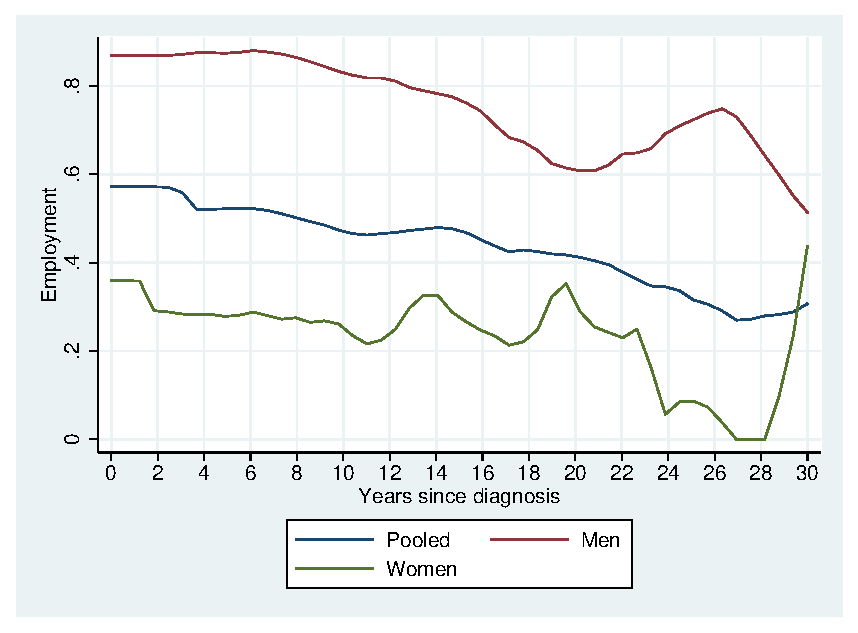
\includegraphics[width=0.5\columnwidth]{figures/lpoly_works_diabetesduration/lpoly_works_diabetesduration.eps}
\end{center}
\end{figure}

\begin{figure}[h!]
\caption{\label{fig:Kernel-weighted-local-polynomial_wage}Kernel-weighted local
polynomial regression of log hourly wages on diabetes duration}%
\begin{center}
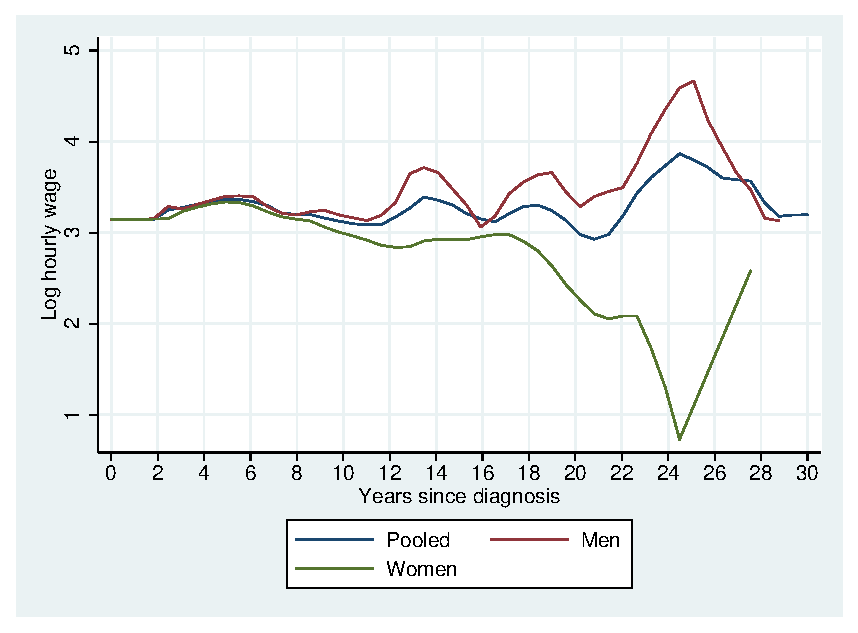
\includegraphics[width=0.5\columnwidth]{figures/lpoly_wage_diabetesduration/lpoly_wage_diabetesduration.eps}
\end{center}
\end{figure}

\begin{figure}[h!]
\caption{\label{fig:Kernel-weighted-local-polynomial_workhrs}Kernel-weighted local
polynomial regression of working hours on diabetes duration}%
\begin{center}
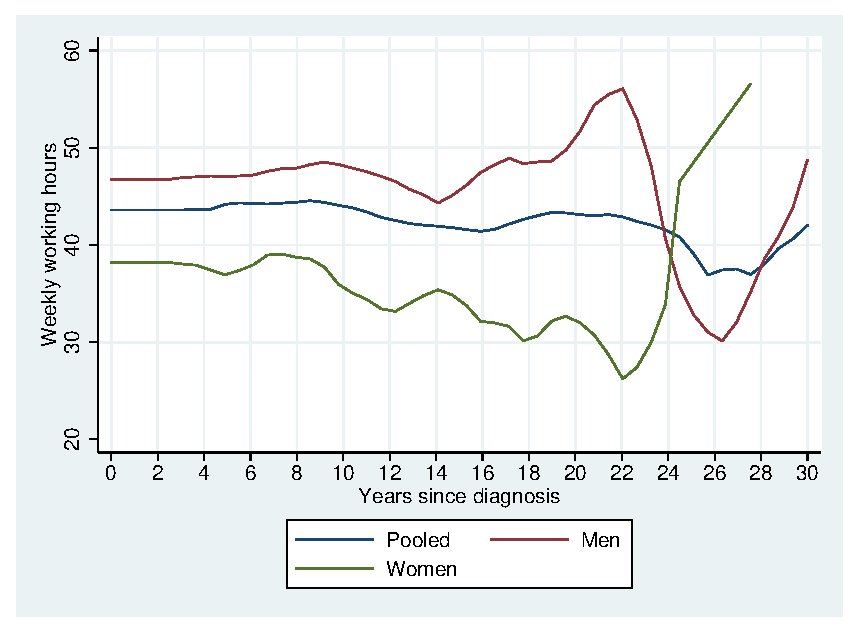
\includegraphics[width=0.5\columnwidth]{figures/lpoly_workhrs_diabetesduration/lpoly_workhrs_diabetesduration.eps}
\end{center}
\end{figure}

\FloatBarrier

Table \ref{tab:Self-reported-diabetes-duration-linear} present the estimations of equations (\ref{eq:duration_linear}) and (\ref{eq:splines}), i.e. the linear and spline models. 

The  results indicate a reduction in employment probability by about 2 percentage points for men with each
additional year since diagnosis. For women the coefficient shows a
reduction of about 1 percentage point per year, though the association
is not as strong. Interestingly, we find a reduction in female wages of about seven percentage points per year with diabetes but no effects for males. There seems to be no relationship between working hours and time since being diagnosed with diabetes.
\begin{table}[h]
\caption{\label{tab:Self-reported-diabetes-duration-linear}Relationship between self-reported years since diagnosis and labor market outcomes using continuous duration and duration splines}
\begin{center}
%\resizebox{\textwidth}{!}{%
\begin{adjustbox}{max width=\textwidth}

{
\def\sym#1{\ifmmode^{#1}\else\(^{#1}\)\fi}
\begin{tabular}{l*{6}{S
S}}
\toprule
                &\multicolumn{2}{c}{Employment}       &\multicolumn{2}{c}{Log hourly wage}&\multicolumn{2}{c}{Monthly work hours}\\\cmidrule(lr){2-3}\cmidrule(lr){4-5}\cmidrule(lr){6-7}
                &\multicolumn{1}{c}{(1)}&\multicolumn{1}{c}{(2)}&\multicolumn{1}{c}{(3)}&\multicolumn{1}{c}{(4)}&\multicolumn{1}{c}{(5)}&\multicolumn{1}{c}{(6)}\\
                &\multicolumn{1}{c}{Males}&\multicolumn{1}{c}{Females}&\multicolumn{1}{c}{Males}&\multicolumn{1}{c}{Females}&\multicolumn{1}{c}{Males}&\multicolumn{1}{c}{Females}\\
\midrule
Panel A (linear) &&&&&&\\
Diabetes duration&    -.021\sym{***}&    -.011\sym{**} &    -.030         &    -.070\sym{**} &     .148         &     .120         \\
                &   (.006)         &   (.005)         &   (.018)         &   (.029)         &   (.338)         &   (.658)         \\
\midrule
Panel B (splines)&&&&&&\\
\hspace*{10mm}0--4&    -.016         &    -.017         &    -.011         &     .036         &     .365         &    1.604         \\
                &   (.012)         &   (.015)         &   (.045)         &   (.117)         &   (.790)         &  (2.289)         \\
\hspace*{10mm}5--11&    -.010         &    -.006         &    -.056         &    -.113\sym{**} &    -.004         &    -.541         \\
                &   (.009)         &   (.008)         &   (.034)         &   (.053)         &   (.594)         &  (1.018)         \\
\hspace*{10mm}12--20&    -.037\sym{**} &    -.017         &     .051         &    -.048         &     .232         &    -.606         \\
                &   (.016)         &   (.011)         &   (.059)         &   (.051)         &   (.933)         &  (1.299)         \\
\hspace*{10mm}> 20&    -.056\sym{*}  &    -.019         &    -.141         &    -.218\sym{***}&     .313         &    8.193\sym{***}\\
                &   (.031)         &   (.018)         &   (.134)         &   (.057)         &  (2.554)         &  (1.720)         \\
N               &    16302         &    22429         &    10774         &     5750         &    13588         &     7394         \\
\bottomrule
\multicolumn{7}{l}{\footnotesize Fixed effects estimation; robust standard errors in parentheses.}\\
\multicolumn{7}{l}{\footnotesize Other control variables: state dummies, urbanisation dummies, education dummies, married dummy,}\\
\multicolumn{7}{l}{\footnotesize number children < 6, wealth, age and calender year fixed effects.}\\
\multicolumn{7}{l}{\footnotesize The wage and working hour models additionally control for type of work (agricultural and self employed}\\
\multicolumn{7}{l}{\footnotesize with non-agricultural employment as the base) and for health insurance status.}\\
\multicolumn{7}{l}{\footnotesize \sym{*} \(p<0.10\), \sym{**} \(p<0.05\), \sym{***} \(p<0.01\)}\\
\end{tabular}
}
%}

\end{adjustbox}
\end{center}
\end{table}  
    
Using the non-linear specification with splines (Table \ref{tab:Self-reported-diabetes-duration-linear}), the
negative association persists for males but not for females. Interestingly, using splines
we find a relatively strong reduction of wages 5-11 years after diagnosis
for women. We also find associations for those with more than 20 years of diabetes, but these estimates may be spurious due to the considerably reduced number of observations, particularly for wages and working hours.

Overall these results suggest a deterioration of the probability of employment and lower earnings for women, in contrast to estimates for the US \citet{Minor2013}, where no such linear relationship is observed. Our non-linear results are not directly comparable to those of \citet{Minor2013}, who uses dummy variables instead of splines and also constructs different duration groups. Minor finds a reduction in employment probabilities of 82 \% points for females after 11 to 15 years and of 60 \% points for males after 2-5 years, indicating very large employment penalties, certainly in comparison to our analysis. \footnote{We estimated a comparable model to that of \citet{Minor2013} using dummy variables and generally find a significant reduction in employment chances throughout, regardless of whether we use our duration groups to construct the dummies or the duration groups used by \citet{Minor2013}. For men, we find a significant reduction of about 6 to 12 percentage points, depending on the used specification, in the first two or four years after diagnosis. In the following years the effect size tends to increase somewhat. For women, we find less evidence for an immediate effect of diagnosis, and  effects do appear after about two years of living with the disease and also increase somewhat over time. These results are available on request.}


\subsection{Cross-sectional biomarker analysis}


In this section we gain additional insights from using the biomarker data collected in the
third wave of the \ac{MxFLS}. As noted in section \ref{sec:Data}, these data enable us to identify respondents with
\ac{HbA1c} levels above the internationally recognized diabetes threshold of 6.4\%, thereby uncovering that 18\% of the biomarker subsample have undiagnosed diabetes. 



\subsubsection*{Biomarkers versus self-reported diabetes}


The results of the complete biomarker analysis are presented in Table \ref{tab:Biomarker_results}. In order to investigate how the subsample of biomarkers compares to the overall sample of the third wave we first estimate a model showing the association of self-reported diabetes with our outcome variables using data of the entire third wave (columns 1--2 and 9--10 in Table \ref{tab:Biomarker_results}). We find similar results to our panel data analysis, if with somewhat smaller coefficients for the association with employment probabilities, particularly for women. Running the same model but using only the data of the biomarker sample (columns 3--4 and 11--12), we find that the coefficient becomes smaller for men and standard errors increase throughout, likely due to the reduction in sample size.

In the next step we investigate the association between biometrically measured
diabetes, irrespective of whether
the condition has or has not been diagnosed, and labor market outcomes, by estimating equation \ref{eq:diab_objective}.\footnote{We include in the indicator for biometrically measured diabetes also those that self-reported a diabetes diagnosis
but had \ac{HbA1c} levels below the diabetes threshold. These people may have good control of their diabetes so that their \ac{HbA1c} levels drop below the threshold and therefore should not be assumed to falsely report a diagnosis. Robustness checks showed that the results were not sensitive to the inclusion of this subpopulation.}  We find evidence for an adverse association of biometrically measured diabetes and the probability of employment
for women and the coefficient is smaller compared with self-reported diabetes. This suggests that relying on self-reported
diabetes exclusively may lead to an upward bias due to those undiagnosed experiencing less pronounced adverse labor market effects.
to account for the differences between the two groups as in equation \ref{eq:diab_sr_ud}, we include both diagnosed and undiagnosed diabetes jointly as independent explanatory variables. We find no association between undiagnosed
diabetes and any labor outcome. For those with diagnosed diabetes, the coefficients for the association with the probability of employment
are close in size and significance to the specification where we account for self-reported diabetes exclusively. Consistent with our earlier findings there is no indication of an association between any form of diabetes and wages or working hours. 
 

\setlength{\tabcolsep}{0pt}
%\begin{landscape}
\begin{table}
\caption{\label{tab:Biomarker_results}Biomarker results}
\begin{center}
\begin{adjustbox}{max width=\linewidth}
{
\def\sym#1{\ifmmode^{#1}\else\(^{#1}\)\fi}
\begin{tabular}{l*{8}{S
S}}
\toprule
                &\multicolumn{2}{c}{Only self-reported (complete sample) }&\multicolumn{2}{c}{Only self-reported (biomarker sample) }&\multicolumn{2}{c}{HbA1c $\geq 6.5\%$ }&\multicolumn{2}{c}{Self-reported and undiagnosed }\\\cmidrule(lr){2-3}\cmidrule(lr){4-5}\cmidrule(lr){6-7}\cmidrule(lr){8-9}
                &\multicolumn{1}{c}{(1)}&\multicolumn{1}{c}{(2)}&\multicolumn{1}{c}{(3)}&\multicolumn{1}{c}{(4)}&\multicolumn{1}{c}{(5)}&\multicolumn{1}{c}{(6)}&\multicolumn{1}{c}{(7)}&\multicolumn{1}{c}{(8)}\\
                &\multicolumn{1}{c}{Males}&\multicolumn{1}{c}{Females}&\multicolumn{1}{c}{Males}&\multicolumn{1}{c}{Females}&\multicolumn{1}{c}{Males}&\multicolumn{1}{c}{Females}&\multicolumn{1}{c}{Males}&\multicolumn{1}{c}{Females}\\
\midrule
\multicolumn{9}{l}{\hspace*{10mm}\textbf{Dependent variable: Employment}} \\
\addlinespace 
Diagnosed diabetes&    -.068\sym{***}&    -.047\sym{***}&    -.049\sym{*}  &    -.043\sym{*}  &                  &                  &    -.048\sym{*}  &    -.048\sym{**} \\
                &   (.017)         &   (.017)         &   (.026)         &   (.023)         &                  &                  &   (.026)         &   (.023)         \\
HbA1c $\geq 6.5\%$&                  &                  &                  &                  &    -.013         &    -.029\sym{*}  &                  &                  \\
                &                  &                  &                  &                  &   (.015)         &   (.017)         &                  &                  \\
Undiagnosed diabetes&                  &                  &                  &                  &                  &                  &     .005         &    -.017         \\
                &                  &                  &                  &                  &                  &                  &   (.019)         &   (.018)         \\
\midrule
R2              &\multicolumn{1}{S}{.091}         &\multicolumn{1}{S}{.102}         &\multicolumn{1}{S}{.079}         &\multicolumn{1}{S}{.108}         &\multicolumn{1}{S}{.078}         &\multicolumn{1}{S}{.107}         &\multicolumn{1}{S}{.079}         &\multicolumn{1}{S}{.108}         \\
N               &\multicolumn{1}{c}{8234}         &\multicolumn{1}{c}{10514}         &\multicolumn{1}{c}{2785}         &\multicolumn{1}{c}{3623}         &\multicolumn{1}{c}{2790}         &\multicolumn{1}{c}{3626}         &\multicolumn{1}{c}{2785}         &\multicolumn{1}{c}{3623}         \\
\midrule
\multicolumn{9}{l}{\hspace*{10mm}\textbf{Dependent variable: Log hourly wages}} \\ 
\addlinespace
Diagnosed diabetes&     .043         &    -.048         &    -.008         &    -.038         &                  &                  &    -.004         &    -.050         \\
                &   (.047)         &   (.072)         &   (.066)         &   (.113)         &                  &                  &   (.068)         &   (.117)         \\
HbA1c $\geq 6.5\%$&                  &                  &                  &                  &     .011         &    -.054         &                  &                  \\
                &                  &                  &                  &                  &   (.044)         &   (.069)         &                  &                  \\
Undiagnosed diabetes&                  &                  &                  &                  &                  &                  &     .018         &    -.052         \\
                &                  &                  &                  &                  &                  &                  &   (.048)         &   (.079)         \\
\midrule
R2              &\multicolumn{1}{S}{.117}         &\multicolumn{1}{S}{.183}         &\multicolumn{1}{S}{.146}         &\multicolumn{1}{S}{.236}         &\multicolumn{1}{S}{.146}         &\multicolumn{1}{S}{.239}         &\multicolumn{1}{S}{.146}         &\multicolumn{1}{S}{.237}         \\
N               &\multicolumn{1}{c}{5515}         &\multicolumn{1}{c}{2887}         &\multicolumn{1}{c}{1803}         &\multicolumn{1}{c}{884}         &\multicolumn{1}{c}{1805}         &\multicolumn{1}{c}{885}         &\multicolumn{1}{c}{1803}         &\multicolumn{1}{c}{884}         \\
\midrule
\multicolumn{9}{l}{\hspace*{10mm}\textbf{Dependent variable: Usual weekly working hours}} \\ 
\addlinespace
Diagnosed diabetes&     .195         &     .395         &    -.338         &    -.780         &                  &                  &    -.301         &    -.176         \\
                &  (1.022)         &  (1.442)         &  (1.286)         &  (2.164)         &                  &                  &  (1.325)         &  (2.216)         \\
HbA1c $\geq 6.5\%$&                  &                  &                  &                  &     .000         &    1.699         &                  &                  \\
                &                  &                  &                  &                  &   (.835)         &  (1.424)         &                  &                  \\
Undiagnosed diabetes&                  &                  &                  &                  &                  &                  &     .160         &    2.635         \\
                &                  &                  &                  &                  &                  &                  &   (.955)         &  (1.838)         \\
\midrule
R2              &\multicolumn{1}{S}{.026}         &\multicolumn{1}{S}{.032}         &\multicolumn{1}{S}{.031}         &\multicolumn{1}{S}{.035}         &\multicolumn{1}{S}{.031}         &\multicolumn{1}{S}{.037}         &\multicolumn{1}{S}{.031}         &\multicolumn{1}{S}{.038}         \\
N               &\multicolumn{1}{c}{6820}         &\multicolumn{1}{c}{3608}         &\multicolumn{1}{c}{2302}         &\multicolumn{1}{c}{1144}         &\multicolumn{1}{c}{2306}         &\multicolumn{1}{c}{1145}         &\multicolumn{1}{c}{2302}         &\multicolumn{1}{c}{1144}         \\
\bottomrule
\multicolumn{9}{l}{\footnotesize Robust standard errors in parentheses; other control variables:age, age squared, state dummies, urbanization dummies, education dummies, married dummy,}\\
\multicolumn{9}{l}{\footnotesize  number children < 6 and wealth;calender year dummies are included as data collection for the third wave was stretched out over several years.}\\
\multicolumn{9}{l}{\footnotesize The wage and working hour models additionally control for type of work (agricultural and self employed with non-agricultural employment as the base)}\\
\multicolumn{9}{l}{\footnotesize and for health insurance status. \sym{*} \(p<0.10\), \sym{**} \(p<0.05\), \sym{***} \(p<0.01\).}\\
\end{tabular}
}

\end{adjustbox}
\end{center}
\end{table}
%\end{landscape}

Overall, the finding that undiagnosed diabetes is not associated with any adverse labor outcomes suggests that the two populations with diabetes, i.e. diagnosed and undiagnosed, are different in ways that are not yet captured by our models. A potential reason may be differences in health between diagnosed and undiagnosed people with diabetes, that affect their employment probabilities. We therefore  add a measure of self-reported health and find that the coefficient of self-reported diabetes is reduced in size and no longer significant for males and only borderline significant for females (Table \ref{tab:Diagnosed_undiagnosed_robust}). Particularly for males reporting bad health is associated with a reduction in employment probabilities while this is not the case for females, suggesting that diagnosed males may actually be in a worse health state, driving the reduction in employment probabilities. For women other factors may play an additional role. Additionally accounting for measures of overweight and obesity, self-reported hypertension, heart disease and insurance status does not further affect the interpretation of the diabetes coefficient (results available on request).

\begin{table}
\caption{\label{tab:Diagnosed_undiagnosed_robust}Diagnosed, undiagnosed diabetes and self-reported health and their association with labor market outcomes (community level fixed effects)}
\begin{center}
\begin{adjustbox}{max width=\linewidth}  
{
\def\sym#1{\ifmmode^{#1}\else\(^{#1}\)\fi}
\begin{tabular}{l*{6}{S
S}}
\toprule
                &\multicolumn{2}{c}{Employment}       &\multicolumn{2}{c}{Log hourly wages} &\multicolumn{2}{c}{Weekly working hours}\\\cmidrule(lr){2-3}\cmidrule(lr){4-5}\cmidrule(lr){6-7}
                &\multicolumn{1}{c}{(1)}&\multicolumn{1}{c}{(2)}&\multicolumn{1}{c}{(3)}&\multicolumn{1}{c}{(4)}&\multicolumn{1}{c}{(5)}&\multicolumn{1}{c}{(6)}\\
                &\multicolumn{1}{c}{Males}&\multicolumn{1}{c}{Females}&\multicolumn{1}{c}{Males}&\multicolumn{1}{c}{Females}&\multicolumn{1}{c}{Males}&\multicolumn{1}{c}{Females}\\

Diagnosed diabetes&    -.032         &    -.040\sym{*}  &     .004         &     .016         &     .111         &    -.668         \\
                &   (.025)         &   (.024)         &   (.069)         &   (.109)         &  (1.374)         &  (2.065)         \\
\addlinespace
Undiagnosed diabetes&     .005         &    -.019         &     .020         &    -.049         &     .119         &    2.753         \\
                &   (.019)         &   (.018)         &   (.049)         &   (.079)         &   (.960)         &  (1.811)         \\                
\multicolumn{6}{l}{Self-reported health status}\\
\hspace*{10mm}good            &     .024         &     .059\sym{*}  &     .066         &    -.115         &   -1.169         &    3.423\sym{*}  \\
                &   (.027)         &   (.035)         &   (.070)         &   (.136)         &  (1.342)         &  (2.054)         \\
\addlinespace
\hspace*{10mm}fair            &    -.005         &     .006         &     .031         &    -.152         &   -1.646         &    4.540\sym{*}  \\
                &   (.026)         &   (.033)         &   (.070)         &   (.141)         &  (1.404)         &  (2.405)         \\
\addlinespace
\hspace*{10mm}bad             &    -.125\sym{**} &    -.025         &    -.018         &    -.376\sym{*}  &   -6.124\sym{**} &    6.882\sym{*}  \\
                &   (.056)         &   (.046)         &   (.174)         &   (.200)         &  (2.678)         &  (3.972)         \\
\addlinespace
\hspace*{10mm}very bad        &    -.167         &     .119         &    -.347\sym{*}  &     .306         &   -1.427         &  -17.360\sym{***}\\
                &   (.127)         &   (.153)         &   (.182)         &   (.433)         &  (3.274)         &  (4.914)         \\
\midrule
R2              &\multicolumn{1}{S}{.089}         &\multicolumn{1}{S}{.111}         &\multicolumn{1}{S}{.148}         &\multicolumn{1}{S}{.244}         &\multicolumn{1}{S}{.035}         &\multicolumn{1}{S}{.048}         \\
N               &\multicolumn{1}{c}{2785}         &\multicolumn{1}{c}{3621}         &\multicolumn{1}{c}{1803}         &\multicolumn{1}{c}{882}         &\multicolumn{1}{c}{2302}         &\multicolumn{1}{c}{1142}         \\
\bottomrule
\multicolumn{7}{l}{\footnotesize Robust standard errors in parentheses.}\\
\multicolumn{7}{l}{\footnotesize Other control variables:age, age squared, state dummies, urbanisation dummies,}\\
\multicolumn{7}{l}{\footnotesize education dummies, married dummy, number children < 6 and wealth.}\\
\multicolumn{7}{l}{\footnotesize Calender year dummies are included as data collection for the third wave was stretched}\\
\multicolumn{7}{l}{\footnotesize out over several years.}\\
\multicolumn{7}{l}{\footnotesize The wage and working hour models additionally control for type of work (agricultural and}\\
\multicolumn{7}{l}{\footnotesize self employed with non-agricultural employment as the base)}\\
\multicolumn{7}{l}{\footnotesize and for health insurance status.}\\
\end{tabular}
}
\end{adjustbox}
\end{center}
\end{table}



\subsubsection{HbA1c levels and labor market outcomes}

The \ac{HbA1c} information in wave 3 also enables us to use it as a proxy for disease
severity and diabetes management. Using three dummy variables for \ac{HbA1c} groups above the
diabetes threshold, i.e. 6.5--7.9, 8--11.9 and 12--14, we investigate
how labor market effects differ when taking \ac{HbA1c} values
into account (table \ref{tab:Self-reported-diabetes-and-hba1clevels}. For brevity we only present the results using community fixed effects here as the results without community fixed effects are similar. For employment probabilities
we again only find adverse associations for
those with diagnosed diabetes, particularly for \ac{HbA1c} levels of 6.5 \% to 7.9\%
and 8\% to 11.9\% compared to people without diabetes and an \ac{HbA1c} below the
diabetes threshold. Given that neither the coefficient size nor significance increases but rather levels off with higher blood glucose levels, we conclude that current diabetes management or severity of diabetes as indicated by \ac{HbA1c} levels is unrelated to the current employment status or any labor market outcome.



\begin{table}[h!]
\caption{\label{tab:Self-reported-diabetes-and-hba1clevels}Diabetes HbA1c levels and labor market outcomes (community level fixed effects)}
\begin{center}
\begin{adjustbox}{max width=\textwidth}
{
\def\sym#1{\ifmmode^{#1}\else\(^{#1}\)\fi}
\begin{tabular}{l*{6}{S
S}}
\toprule
                &\multicolumn{2}{c}{Employment}       &\multicolumn{2}{c}{Log hourly wages}&\multicolumn{2}{c}{Weekly working hours}\\\cmidrule(lr){2-3}\cmidrule(lr){4-5}\cmidrule(lr){6-7}
                &\multicolumn{1}{c}{(1)}&\multicolumn{1}{c}{(2)}&\multicolumn{1}{c}{(3)}&\multicolumn{1}{c}{(4)}&\multicolumn{1}{c}{(5)}&\multicolumn{1}{c}{(6)}\\
                &\multicolumn{1}{c}{Males}&\multicolumn{1}{c}{Females}&\multicolumn{1}{c}{Males}&\multicolumn{1}{c}{Females}&\multicolumn{1}{c}{Males}&\multicolumn{1}{c}{Females}\\
\midrule
\multicolumn{6}{l}{Self-reported diabetes} \\
6.5 $\leq$ HbA1c < 8&    -.130\sym{**} &    -.068         &    -.211\sym{*}  &     .003         &    1.878         &   -5.682         \\
                &   (.056)         &   (.049)         &   (.122)         &   (.245)         &  (2.727)         &  (4.797)         \\
8 $\leq$ HbA1c < 12&    -.051         &    -.104\sym{***}&     .040         &     .026         &   -2.193         &   -1.369         \\
                &   (.033)         &   (.032)         &   (.091)         &   (.167)         &  (1.861)         &  (3.341)         \\
HbA1c $\geq 12$       &     .015         &    -.027         &    -.103         &    -.291         &    -.361         &    -.676         \\
                &   (.046)         &   (.049)         &   (.143)         &   (.230)         &  (3.071)         &  (3.603)         \\
\multicolumn{6}{l}{Undiagnosed diabetes} \\                
6.5 $\leq$ HbA1c < 8&     .018         &     .002         &     .020         &    -.037         &     .928         &    3.710         \\
                &   (.021)         &   (.025)         &   (.058)         &   (.094)         &  (1.175)         &  (2.318)         \\
8 $\leq$ HbA1c < 12&     .011         &    -.018         &     .011         &    -.146         &   -1.016         &    -.437         \\
                &   (.037)         &   (.031)         &   (.078)         &   (.134)         &  (1.511)         &  (2.716)         \\
HbA1c $\geq 12$     &     .008         &    -.062         &    -.018         &     .183         &   -1.740         &    1.591         \\
                &   (.042)         &   (.045)         &   (.087)         &   (.185)         &  (2.100)         &  (4.066)         \\
\midrule
R2              &\multicolumn{1}{S}{.026}         &\multicolumn{1}{S}{.079}         &\multicolumn{1}{S}{.146}         &\multicolumn{1}{S}{.232}         &\multicolumn{1}{S}{.029}         &\multicolumn{1}{S}{.040}         \\
N               &\multicolumn{1}{c}{2785}         &\multicolumn{1}{c}{3623}         &\multicolumn{1}{c}{1804}         &\multicolumn{1}{c}{885}         &\multicolumn{1}{c}{2305}         &\multicolumn{1}{c}{1145}         \\
\bottomrule
\multicolumn{7}{l}{\footnotesize Robust standard errors in parentheses.}\\
\multicolumn{7}{l}{\footnotesize Other control variables:age, age squared, state dummies, urbanisation dummies,}\\
\multicolumn{7}{l}{\footnotesize education dummies, married dummy, number children < 6 and wealth.}\\
\multicolumn{7}{l}{\footnotesize Calender year dummies are included as data collection for the third wave was stretched}\\
\multicolumn{7}{l}{\footnotesize out over several years.}\\
\multicolumn{7}{l}{\footnotesize The wage and working hour models additionally control for type of work (agricultural and}\\
\multicolumn{7}{l}{\footnotesize self employed with non-agricultural employment as the base)}\\
\multicolumn{7}{l}{\footnotesize and for health insurance status.}\\
\end{tabular}
}
\end{adjustbox}
\end{center}
\end{table}

To the best of our knowledge only one study has previously used biomarker data to analyze the relationship with labor market outcomes in a comparable population. \citet{BrownIII2011} use data for a Mexican American
population in a broadly comparable way to this paper, though stopping short of investigating
the labor market impact of undiagnosed diabetes. The study indicates
an increasing negative relationship of diabetes and employment
probabilities and wages for men as \ac{HbA1c} levels increased, interacting \ac{HbA1c} levels
with the diabetes dummy.\footnote{We estimated a similar model but
do not find any indication that increasing \ac{HbA1c} levels were
related with employment probabilities (results available on request).} We
find the same to be true when using indicator variables for different
\ac{HbA1c} groups above the diabetes threshold, where the main effects
are found for those with relatively well managed diabetes and no
effects for those with the highest \ac{HbA1c} levels. While we cannot explain these differences in the results between our study and the study of \citet{BrownIII2011} other than by acknowledging the fact that our study is located in a very different country and uses a different age group, other results in their study were reasonably in line with our findings that once people are diagnosed with diabetes, current diabetes management plays a minor role in determining labor market outcomes. This is not surprising given that \ac{HbA1c} levels only provide a picture of blood glucose levels over the last three month. They therefore may not be representative of blood glucose levels in the years before and after the diabetes diagnosis which ultimately determine how soon complications appear and how severe they will be.

\section{\label{sec:Conclusion}Conclusion}

According to the relatively novel panel data used here, self-reported diabetes has increased in Mexico between 2002 and 2012, and overall
diabetes prevalence has reached worrying
levels, in particular when including the strikingly large share of the undiagnosed diabetes population that we are able to investigate in this analysis. In light of the rising importance of diabetes in Mexico and other \ac{MICs}, the demand for  thus far extremely scarce evidence on the associated economic consequences has been large. We contribute to filling this gap by providing important additional evidence on the globally much under-researched labor market effects of diabetes, taking into account several complexities that arise due the nature of the disease.

Our first important finding is the confirmation of a considerable employment burden for men and women reporting a diabetes diagnosis, even after accounting for an important source of potential unobserved heterogeneity by using individual \ac{FE} for the first time in the investigation of diabetes labor market effects. We see this as a potentially more valid strategy than relying on the at least questionable \ac{IV} strategies used so far in the literature. This strategy also allowed us to account for any sample selection into employment based on time-invariant heterogeneity such as innate ability. We find that diabetes very likely is not related to a decrease in wages or working hours, suggesting that people who receive a diabetes diagnosis often drop out of the labor market once debilitating diabetes related complications appear that would limit their work performance. This is of particular relevance in jobs where formal job protection and good access to healthcare may be less available and that are also relatively more strenuous. However, those who remain employed do not appear to suffer any wage or labor supply effects, possibly because they are still relatively healthy or they are able to resort to a type of work were their diabetes does not inhibit their performance. Future research will be needed to confirm and further investigate this finding and interpretation.

Using the same strategy we also investigate the effect of diabetes duration on labor market outcomes and find that diabetes likely has a continuous adverse relationship with employment probabilities, which might become increasingly stronger after the first ten years since diagnosis. This is not surprising given that many complications of diabetes only appear after some time of living with the disease. This likely bodes ill for many countries were diabetes, and in particular Type 2???diabetes starts appearing at an increasingly younger age in recent years, causing people to live with the disease for larger parts of their productive lifespan, possibly exacerbating the economic effects of unemployment due to diabetes. 

The other main contribution of this paper is the ability to identify previously unobserved people with diabetes via the use of biomarker data and the finding that undiagnosed
diabetes is not associated with labor market outcomes in Mexico. We still mostly find a negative association of diabetes with labor market outcomes but this association is significantly reduced. While this is only a cross-sectional analysis and the results can only be interpreted as associations, this is still an indication that studies relying solely on self-reported diabetes may not under- but overestimate the effect of diabetes on labor market outcomes due to non-classical reporting error. Therefore, it is important to consider the population of people with diabetes as consisting of those with self-reported diabetes and those with undiagnosed diabetes, where the former differs from the latter in the amount of health information they possess and likely also their health status. The best way then to analyze the effects of diabetes should be to, if possible, explicitly account for both groups, as using an \ac{IV} strategy will not correct for non-classical measurement error \citep{Cawley2015}.

Several limitations of this study exist. First, we are not able to investigate directly to what extend the psychological effect of a diabetes diagnosis might affect employment probabilities due to justification bias.\footnote{Another potential problem may be that the \ac{HbA1c} measurements are upward biased as a result of the used technical device Bio-Rad in2it, which has been shown to correlate strongly with laboratory measurements \citep{HealthQualityOntario2014} but had also been found by one study to produce somewhat higher \ac{HbA1c} estimates \citep{Yeo2009}. This could cause many people just above the diabetes threshold to be falsely qualified as having undiagnosed diabetes, potentially attenuating the estimates. To test this, we reestimated above models using an alternative diabetes threshold of $\ac{HbA1c} \geq 7$. The results, however, remained similar, not providing evidence for an attenuation bias due to misclassification.}

To reiterate, the study finds a considerable negative impact of self-reported diabetes on employment probabilities, a finding that is likely also of relevance to other \ac{MICs} facing similar diabetes problems. Further, when estimating any effects of diabetes using self-reported measures, any conclusions drawn should be limited to those already diagnosed as otherwise any effects are likely to be overstated due to the often large population with undiagnosed diabetes. 


\begin{appendix}
\clearpage


\part*{\label{part:Appendix}Appendix}

\section{\label{sec:Appendix}Strategies to deal with measurement error}

As discussed above, reporting error is likely to pose a considerable
challenge in the use of self-reported data. Fortunately, the \ac{MxFLS}
data provides several possibilities to assess the amount of misreporting
as well as to partly correct for it, in the attempt to reduce any resulting
bias when estimating the labor market effects of diabetes. In what
follows we describe our approach of dealing with inconsistencies in
self-reported diabetes over time.

One of the key advantages of panel data is in its repeated measurement
for many of the individuals, thereby allowing to uncover inconsistencies
for those individuals with at least two observations. While we are
not aware of any literature investigating the issue of inconsistencies
in self-reported diabetes over time, a study by \citet{Zajacova2010}
on the consistency of a self-reported cancer diagnosis over time in
a USA population found that 30 percent of those who had reported a
cancer diagnosis at an earlier point, did report at a later point
that they never had received a cancer diagnosis. They also found that
a more recent diagnosis was reported with greater consistency possibly
due to increasing recall problems and/or reduced salience as time
since diagnosis progresses.

We find similar inconsistencies in the diabetes self-reports over
the three waves of the \ac{MxFLS} data, with between 10 to 20 percent
of those reporting diabetes in one wave not reporting diabetes in
one of the subsequent waves. In order to correct these inconsistencies we were interested in the validity of diabetes self-reports. While we could not find a study assessing
the validity of self-reported diabetes in Mexico, a study from China
has shown that specificity of self-reported diabetes - meaning that
those who self-report a diabetes diagnosis actually have diabetes
- was very high (>98 percent for China), while sensitivity - a measure
of how many people with diabetes, diagnosed or undiagnosed, actually
self-report the disease - was low (40 percent for China) \citep{Yuan2015}.
This indicates that people who report a diabetes diagnosis are likely
to indeed have the condition while many of those not reporting
a diabetes diagnosis could have diabetes as well but are unaware.

Thanks to the biomarker data provided in the third wave of the \ac{MxFLS},
we are also able to assess the validity of self-reported diabetes
by using \ac{HbA1c} levels and the self-reports of diabetes
related medicine use. The \ac{WHO}
recommends a cut-off value of an \ac{HbA1c} $\geq6.5$ percent
to diagnose a person with diabetes \citep{WorldHealthOrganization2011}.
Of the subsample selected for biomarker measurements and answering
the diabetes question (n=6895), 705 reported a diabetes diagnosis
and of those 632 (90 percent) had an \ac{HbA1c} $\geq6.5$ percent
or did report taking diabetes medication, indicating relatively high specificity in our data as well.

We therefore assumed for people with information from only two waves, that if
they reported a diabetes diagnosis in a prior wave they also had diabetes
in the ensuing wave even if they did not report a diabetes diagnosis.
For people where we had data from all three waves, we used that
additional information to make a decision on how to deal with inconsistencies
using the rules outlined in Table \ref{tab:Inconsistencies}:

\begin{table}[h!]
\caption{\label{tab:Inconsistencies}Inconsistencies in diabetes self-report in MxFLS}
\begin{center}
\begin{adjustbox}{max width=\textwidth}
\begin{tabular}{llc}
\hline 
Inconsistency  & Assumption  & Number of observations replaced\tabularnewline
\hline 
Diabetes self report in 2002, 2005 but not in 2009  & Has diabetes in 2009 as well  & 34\tabularnewline
Diabetes self report in 2002, 2009 but not in 2005  & Has diabetes in 2005 as well  & 94\tabularnewline
Diabetes self report only in 2002, but not in 2005 and 2009  & Has no diabetes in 2002 either  & 86\tabularnewline
Diabetes self report only in 2005, but not in 2002 and 2009  & Has no diabetes in 2005 either  & 71\tabularnewline
Diabetes self report in 2002, but not in 2005. Not in survey in 2009  & Has diabetes in 2005 as well  & 43\tabularnewline
Diabetes self report in 2005, but not in 2009. Not in survey in 2002  & Has diabetes in 2009 as well  & 32\tabularnewline
\end{tabular}
\end{adjustbox}
\end{center}
\end{table}


This approach should add more consistency to the self-reported diabetes
information by using all available information. We tested if the results
of the \ac{HbA1c} tests for the subpopulation in 2009 with biomarker
information and inconsistencies in their diabetes reporting (n=96,
48 with two and 48 with one self-report of diabetes) would support
this decision. Therefore we compared the mean \ac{HbA1c} values for those
who had two self-reports of a diagnosis of diabetes in the full three
waves with those with only one self-report. Using a t-test we found
a significantly (p<0.001) higher mean \ac{HbA1c} of 9.6 percent
for those with two self-reports compared to 7.0 percent for those
with only one self-report of diabetes. Further, of those with one
self-report, only 30 percent had an \ac{HbA1c}$\geq6.5$ percent
compared to 87 percent of those with two self-reports. Bases on these results we were reassured that the way we have dealt with the inconsistencies in the data should
minimize misclassification of people into diabetes or no-diabetes
and should reduce some of the measurement error in the diabetes data. Unfortunately we cannot use a similar method for dealing with inconsistencies
in the self-reported year of diabetes diagnosis as it has only been reported once. Hence, the results from models using
duration of diabetes instead of self-reported diabetes must be interpreted
particularly carefully.

\end{appendix}

Acknowledgement

We are grateful to the participants at the European Health Economics Association PhD-Supervisor conference September 2015 in Paris, the Health, Education and Labor Market Outcomes Workshop at the WifOR Institute in October 2015 in Darmstadt, Germany, seminar participants at the Centre for Health Economics at York University, and Max Bachmann for helpful comments.


\noindent \bibliographystyle{elsarticle-harv} 

%\addbibresource{/home/till/Dokumente/BibTex/Second_Mexico_paper-Article.bib}

\bibliography{/home/till/Dokumente/BibTex/Second_Mexico_paper-Article}
\end{document}

